\subsection{Functional Features}
	This tool is designed to allow an inexperienced animator to see results quickly.  Experienced developers will also benefit from the ability to quickly get animations going in order to iterate on ideas quickly.  
	Animations are composed one or more of drawn paths called a Line of Action (LOA).  With this tool the user will be able to:
\begin{itemize}
	\item Draw a LOA.
	\item Edit a previously drawn LOA.
	\item Select a mesh that the animation will be applied to.
	\item Preview the animation.
	\item Layer animations together into one animation.
	\item Save/Load animations.
	\item Export an animation into a standard format.
\end{itemize}
\subsubsection{Interface}
\begin{figure}[H]
\centering
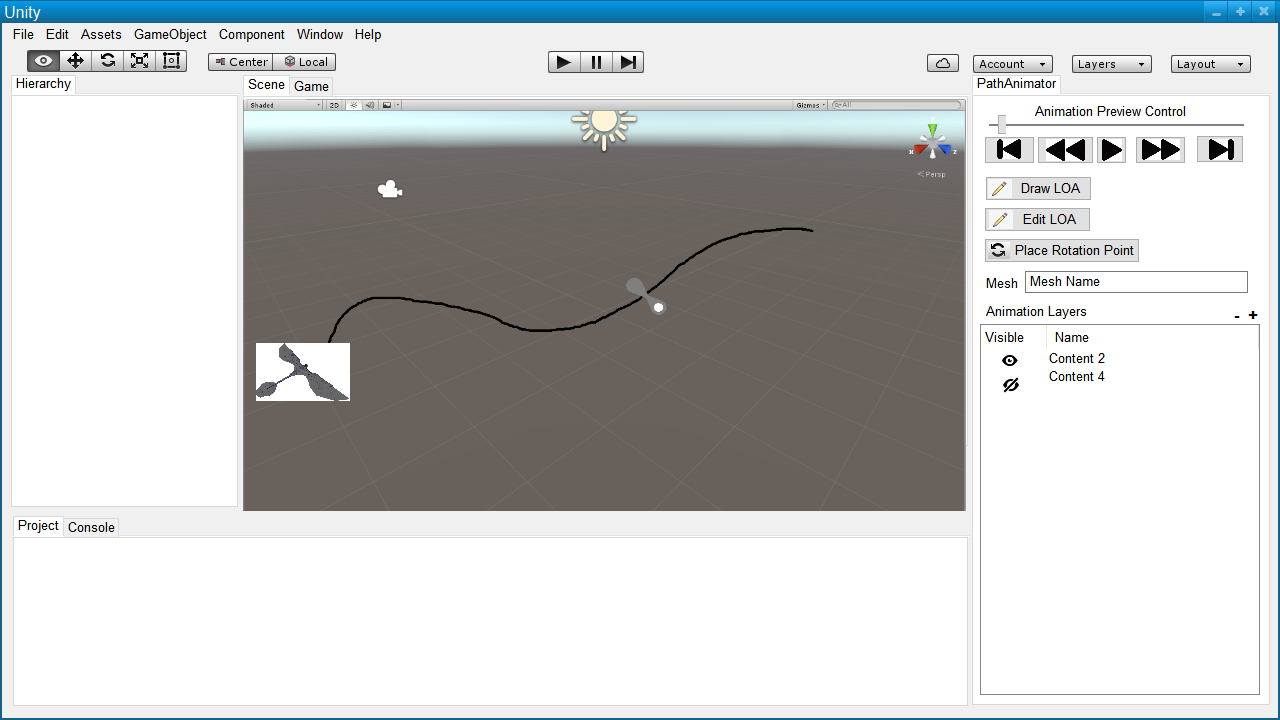
\includegraphics[scale=0.25]{MainInterface}
\caption{Mockup of the main interface, integrated into Unity}
\label{fig:interface}
\end{figure}
This tool will be used as a plugin to Unity.  Therefore, the interface will be integrated into the Unity user interface.  Figure~\ref{fig:interface} shows a mock up of how the tool will look integrated with the Unity user interface.

There are two components to the user interface: the control panel, and the view panel.  Each will be explained in detail in the following sections.
\begin{figure}[H]
\centering
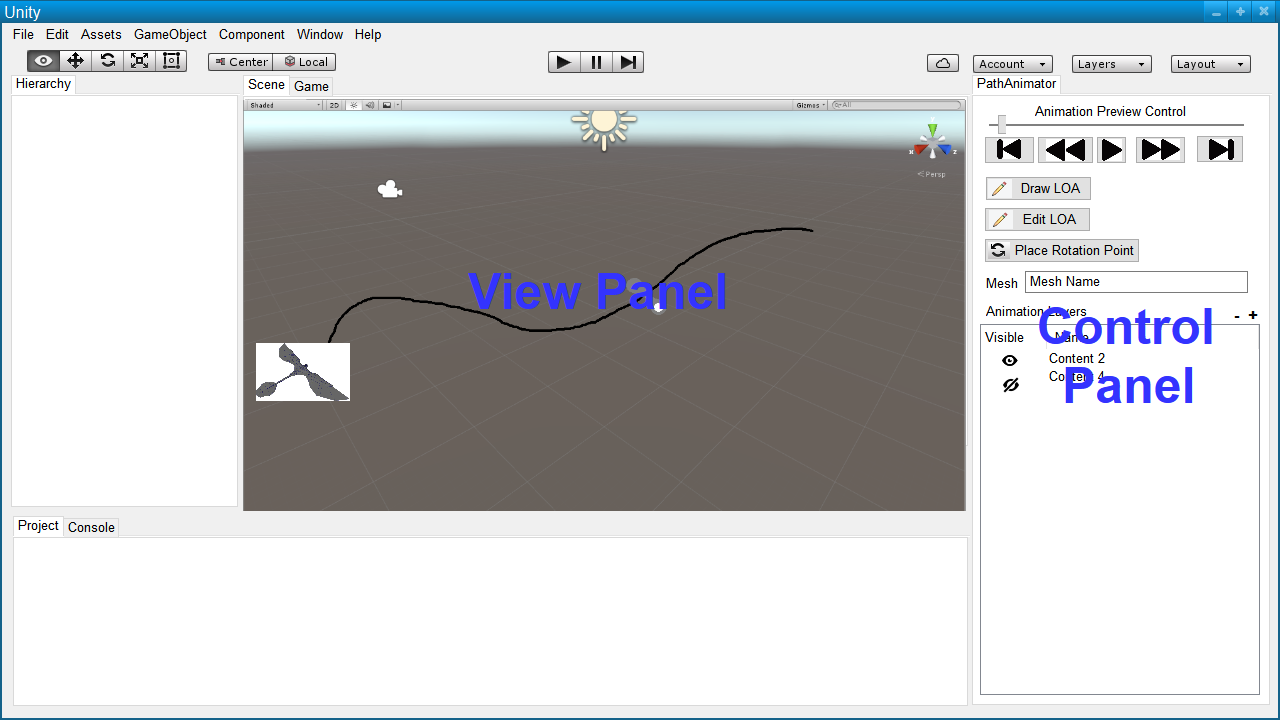
\includegraphics[scale=0.25]{MainInterfaceLabled}
\caption{Sections of the Unity user interface that are included with the plugin}
\label{fig:interfaceLabled}
\end{figure}
\subsubsection{Control Panel}
\begin{figure}[H]
\centering
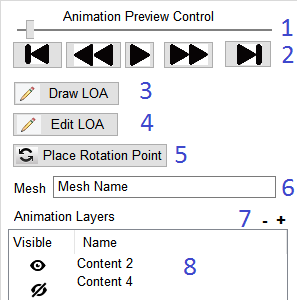
\includegraphics{ControlPanel}
\caption{The control panel}
\label{fig:controlPanel}
\end{figure}
Figure~\ref{fig:controlPanel} shows the control panel.  The function of each component is described below.
\begin{enumerate}
	\item \textbf{Animation Preview Scrubber} \hfill \\
		Allows the user to go to any point in the animation.  The position of the mesh at that point in the animation will be shown in the view panel.
	\item \textbf{Animation preview controls} \hfill \\
		With these controls a user can play, pause, restart, rewind, fast forward, and go to the end of the animation.
	\item \textbf{Draw LOA} \hfill \\
		When this button is clicked the plugin goes into LOA drawing mode.
	\item \textbf{Edit LOA} \hfill \\
		When this button is clicked the plugin goes into LOA edit mode.
	\item \textbf{Place Rotation Point} \hfill \\
		When this button is clicked the user will be able to place rotation points on the LOA.
	\item \textbf{Mesh} \hfill \\
		This component is used to select the mesh that the animation will be applied to.
	\item \textbf{Add/Remove animation layers} \hfill \\
		These buttons allow the user to add or remove animations that will be layered into the overall animation.
	\item \textbf{Animation Layers grid} \hfill \\
		This grid shows the animation layers currently applied in this contained in the overall animation.  The user can set the visibility of each layer.
\end{enumerate}
\subsubsection{View Panel}
\begin{figure}[H]
\centering
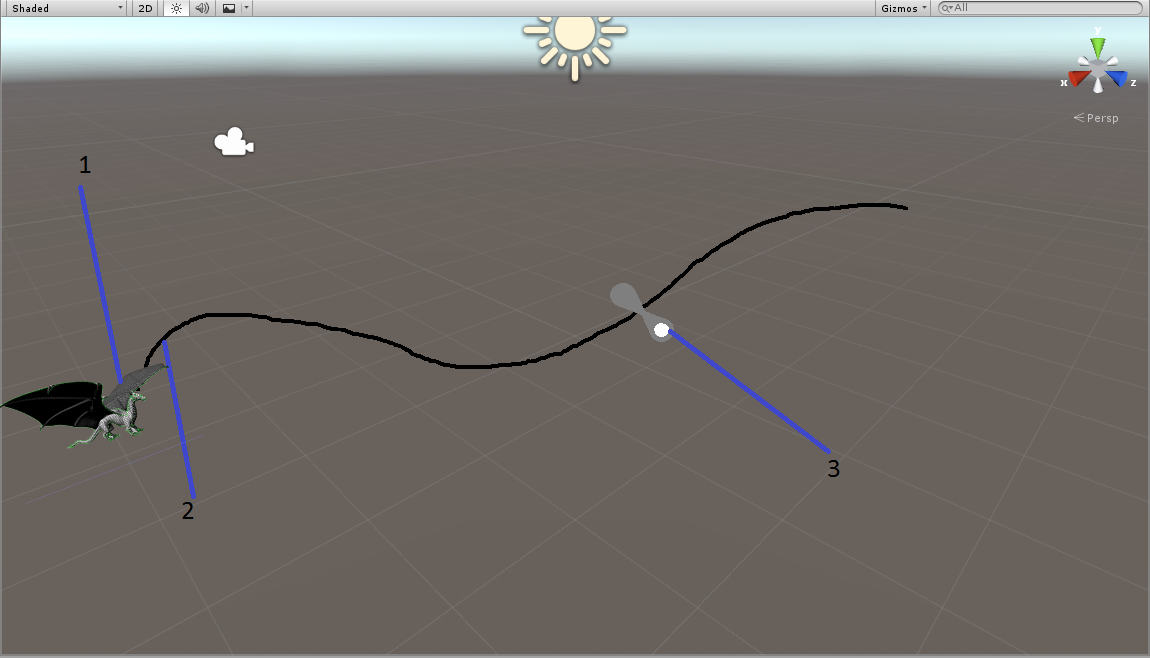
\includegraphics[scale=0.45]{ViewPanel}
\caption{The view panel}
\label{fig:viewPanel}
\end{figure}
Figure~\ref{fig:viewPanel} shows the view panel.  The function of each component is described below.
\begin{enumerate}
	\item \textbf{Mesh} \hfill \\
		The Mesh is displayed in the position corresponding to the current frame of the animation.
	\item \textbf{LOA} \hfill \\
		All LOAs that have been drawn will be displayed.
	\item \textbf{Rotation Point} \hfill \\
		This is a rotation point.  It will be oriented according to the rotation that will be applied to the mesh.
\end{enumerate}
\subsubsection{Line of Action Drawing}
	When the user clicks the "Draw LOA" button, the plugin enters LOA drawing mode.  In this mode the user will draw the LOA in the view panel.  The user may draw multiple LOAs.  How fast the line is drawn as well as the composition of the line will factor into the animation(Position, rotation, stretch, skew).  Multiple LOAs will further refine the animation.
	When the user clicks the "Edit LOA" button, the plugin enters LOA editing mode.  In this mode the user can select a LOA and either delete it or redraw it.
\subsubsection{Rotation Points}
	The user can add a rotation point to any point on a LOA.  The rotation point will have a specific rotation vector.  This rotation vector will influence the rotation of the mesh when it reaches the rotation point.  The rotation vector can be edited by selecting the rotation point and dragging in the desired direction.
\subsubsection{Animation Layering}
	Animations can be layered into one animation.  Each layer has its own LOAs and rotation points associated with it.  When the animations are layered the overall animation will be interpolated using all of the animation layers.
\subsubsection{Exporting}
	When the artist is satisfied with the animation they have created they will have the ability to export it into a format that will be usable in other applications.
